\documentclass[9pt,twoside,lineno]{pnas-new}
% Use the lineno option to display guide line numbers if required.

\templatetype{pnassupportinginfo}
% \readytosubmit %% Uncomment this line before submitting, so that the instruction page is removed.

\title{Conceptualizing and Measuring Resilience to Hazards as Access to Essential Services}
\author{T M Logan and S D Guikema}
\correspondingauthor{T Logan\\E-mail: tomlogan@umich.edu}

\begin{document}

%% Comment/remove this line before generating final copy for submission
% \instructionspage  

\maketitle

%% Adds the main heading for the SI text. Comment out this line if you do not have any supporting information text.
\SItext

\section*{Mapping the access distribution to a resilience curve}

Figure \ref{fig:cdf_to_res} conceptually demonstrates how the distribution of access is mapped to a resilience curve. The four time-states show the progression through the hazard cycle, from pre-disruption, disruption, recovery, and then transformation with future mitigation. Quantifying access to essential services has advantages throughout the hazard cycle that are discussed later in this section. Fundamentally, it allows us to assess the capacity of the system to maintain and restore desired functionality following a disruption. 


\begin{figure}
    \centering
    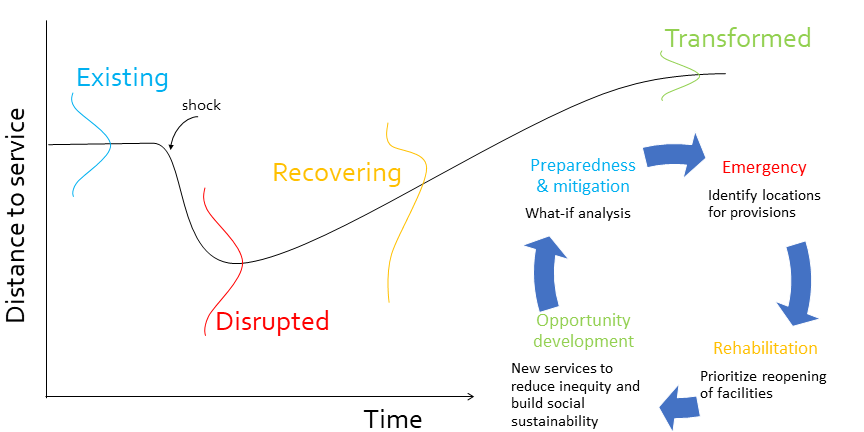
\includegraphics[width=\linewidth]{report/fig/Figure_2.png}
    \caption{
    Comparison of predictive accuracy between the different models.
    }
    \label{fig:cdf_to_res}
\end{figure}



%%% Each figure should be on its own page
% \newpage
%  \begin{table}
%      \centering
%      \includegraphics[width=\linewidth]{report/figures/summary_stats.png}
%      \caption{Summary statistics of the variables included in our analysis.}
%      \label{tab:summary_statistics}
%  \end{table}



\end{document}